% TeX encoding = utf8
% TeX spellcheck = pl_PL 
\documentclass[a4paper, 12pt]{article}
\usepackage[utf8]{inputenc}
\usepackage[polish]{babel}
\usepackage{polski}
\usepackage{graphicx}
\usepackage{listings}
\usepackage{amsfonts}
\usepackage{amsmath}
\usepackage{geometry}
\usepackage{indentfirst}
\usepackage{subfigure}
\usepackage{url}
\usepackage{listings}
\usepackage{color}

%\newgeometry{tmargin=2.5cm, bmargin=2.5cm, lmargin=3.5cm, rmargin=2.5cm}
\setcounter{secnumdepth}{2}
\setlength{\fboxsep}{0pt}
\lstset{language=C++,
                basicstyle=\ttfamily,
                keywordstyle=\color{blue}\ttfamily,
                stringstyle=\color{red}\ttfamily,
                commentstyle=\color{green}\ttfamily,
                morecomment=[l][\color{magenta}]{\#}
}

\author{Jakub Postępski}
\title{Pracownia dyplomowa I}
\graphicspath{ {images/} }

\begin{document}
	\maketitle
	\section{Wstęp}
	\subsection{Zarys pracy}
	Wynikiem tej pracy inżynierskiej ma być zrealizowanie oprogramowania, przy pomocy którego komunikować będą się podzespoły robota mobilnego Elektron. 
	\subsection{Opis robota}
	Instytut Automatyki i Informatyki Stosowanej posiada trzy roboty Elektron, które służą jako pomoc dydaktyczna. Konstrukcja ta jest platformą o napędzie różnicowym, relalizowanym przez dwa silniki elektryczne. Każdy z nich sprzężony jest z trzema kołami, lewymi bądź prawymi. Ich pracę bezpośrednio nadzoruje sterownik silników z mikrokontolerem dsPIC33FJ32MC302, posiadającym port komunikacyjny RS-485. Sterownik pokazany jest na rysunku \ref{img:sterownikSilnikow}. Głównym modułem decyzyjnym jest umieszczony w obudowie robota komputer klasy PC, z procesorem Intel Atom, dyskiem SSD oraz systemem Ubuntu z zainstalowanym ROSem. Po odpowiedniej konfiguracji robot może być podłączony do sieci wi-fi. Można też do niego podłączyć różne peryferia takie jak Microsoft Kinect. Robot zasilany jest z zestawu baterii, ładowanych przy pomocy zasilacza 24V. \par
	Robot wyposażony jest w główny sterownik, przedstawiony na rysunku \ref{img:glownySterownik}, który posiada łącza komunikacyjne z różnymi częściami robota. W szczególności to z tym modułem komunikuje się komputer centralny oraz sterownik silników, lecz może on też sterować pracą innych peryferiów. Dodatkowo sterownik ten zarządza zasilaniem robota, ma wbudowany wyświetlacz LCD, zestaw przekaźników mocy oraz cztery przyciski monostabilne. Sterownik ten posiada mikrokontroler STM32F107VCT.\par
	Robot zaprezentowany jest na rysunku \ref{img:elektron}.
	\begin{figure}[ht]
	    \centering
	    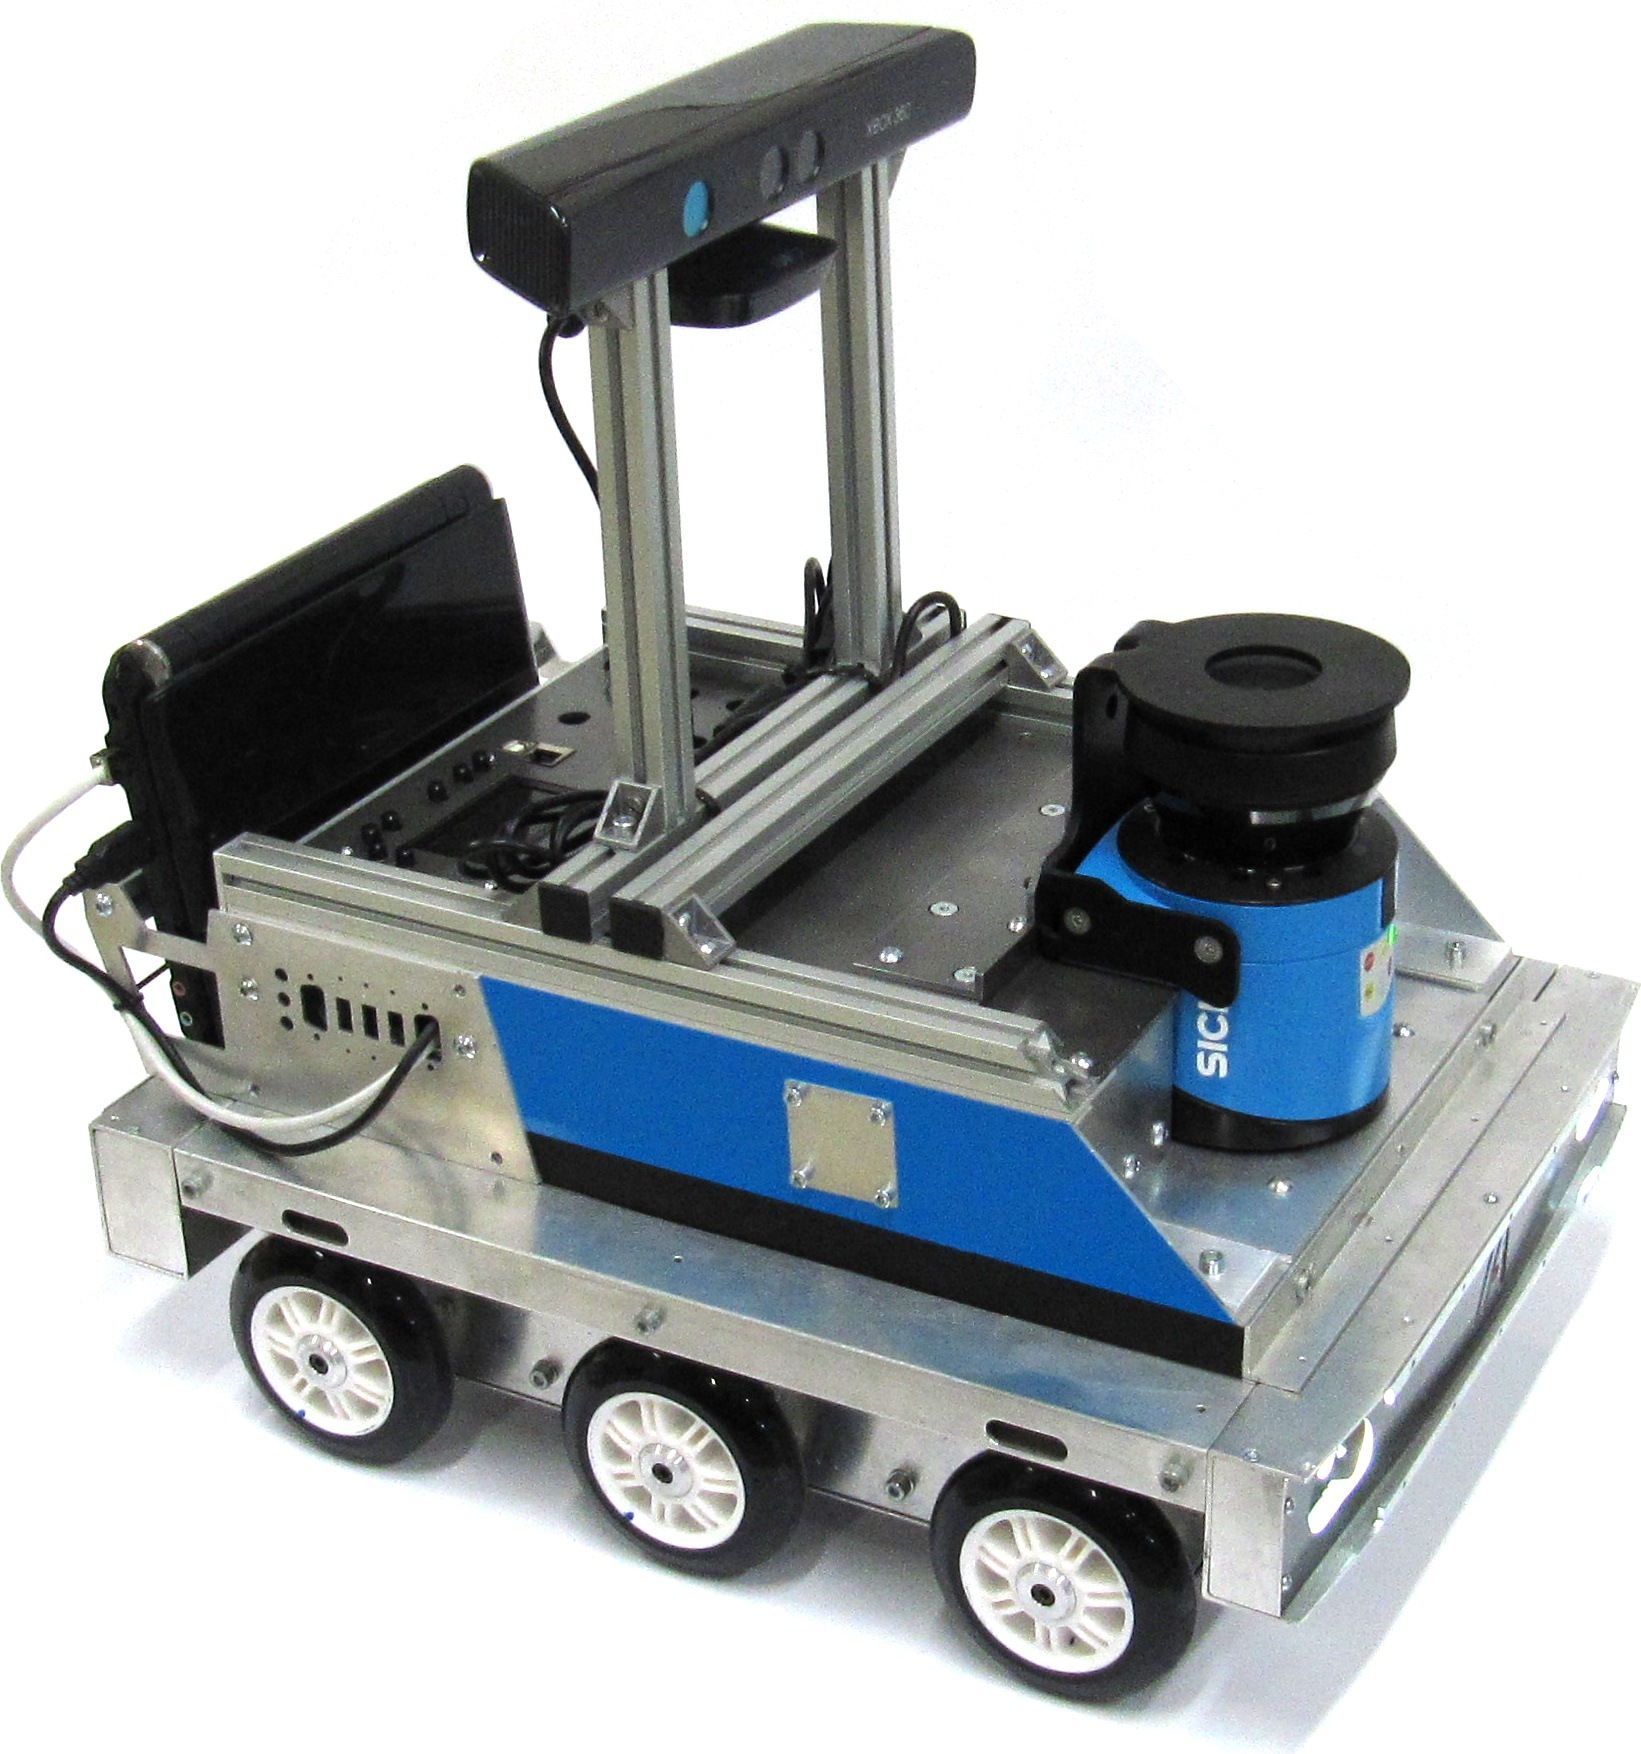
\includegraphics[width=0.4\textwidth]{elektron}
	    \caption{Zdjęcie jednego z robotów Elektron. Źródło\cite{ElektronRobotyka}.}
	    \label{img:elektron}
	\end{figure}
	\begin{figure}[ht]
	    \centering
	    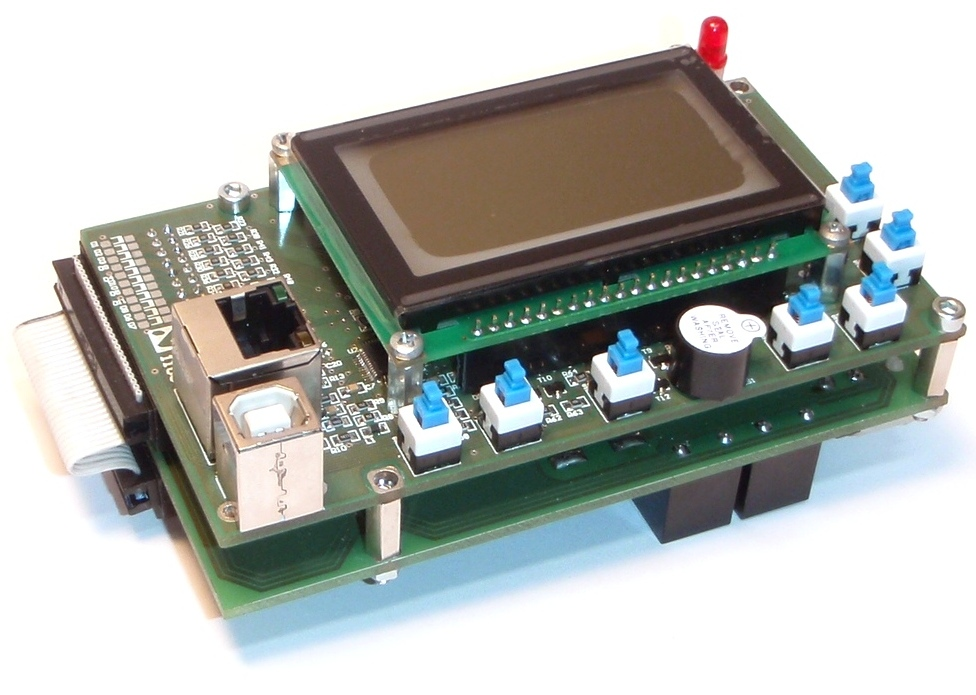
\includegraphics[width=0.4\textwidth]{main}
	    \caption{Główny sterownik robota, kontrolowany, przez STM32F107. Źródło\cite{ElektronRobotyka}.}
	    \label{img:glownySterownik}
	\end{figure}
	\begin{figure}[ht]
	    \centering
	    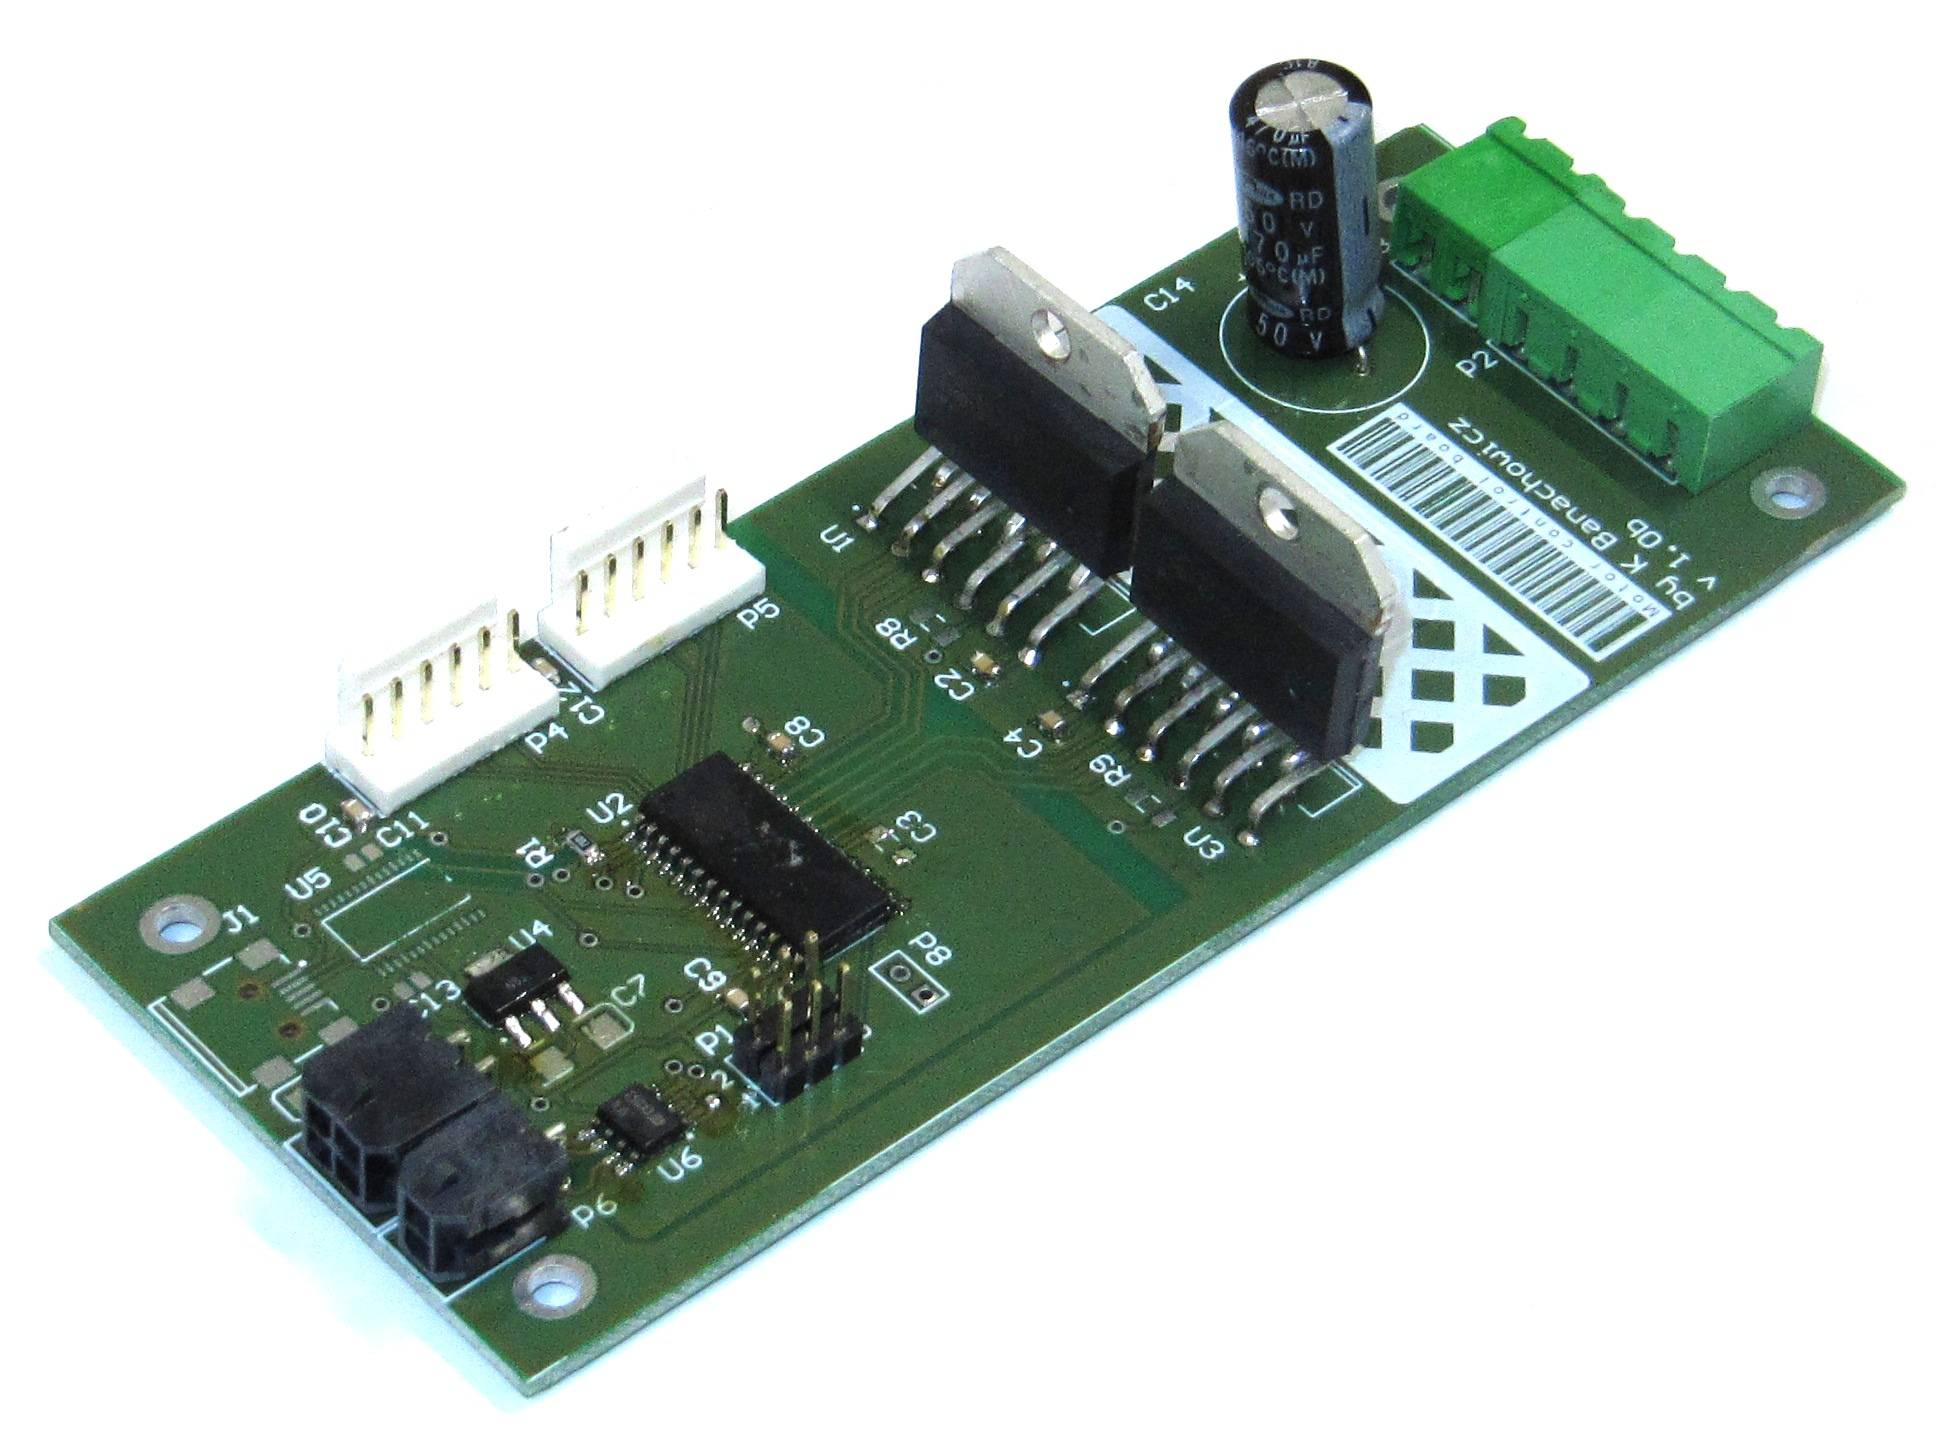
\includegraphics[width=0.4\textwidth]{sterownik}
	    \caption{Sterownik silników robota, kontrolowany przez dsPIC33FJ32MC302. Źródło\cite{ElektronRobotyka}.}
	    \label{img:sterownikSilnikow}
	\end{figure}
	\subsection{Motywacja}
	Wykonanie niezawodnego i odpowiednio szybkiego oprogrowania może spowodować wzrost użyteczności robotów Elektron, a więc ułatwić pracę innym studentom. Dodatkową zachętą dla autora  jest możliwość nauki systemów robotycznych. Jest to też dobra okazja, aby zdobyć doświadczenie w programowaniu mikrokontrolerów firmy ST oraz pracy ze sprzętem wykorzystywanym w robotyce mobilnej. 
	\section{Wymagania stawiane pracy}
	Głównym celem pracy ma być wytworzenie oraz opis rozwiązania, które pozwoli na szybką, deterministyczną i niezawodną komunikację pomiędzy komputerem centralnym oraz głównym sterownikiem z mikrokontrolerem STM32F107. Konsekwencją takiego działania ma być sprawny nadzór podzespołów Elektrona, z których najważniejsza jest transmisja sterowania silników. Działania w początkowej fazie mają być prowadzone na robocie Elektron 3. W przypadku pomyślnego ich ukończenia, istnieje szansa, że wszystkie trzy roboty Elektron zostaną zmodyfikowane w ten sam sposób. Wykonywane działania mają w praktyce objąć napisanie programu dla mikrokontrolera STM32F107, oraz odpowiedniej biblioteki dla systemu Ubuntu. Biblioteka ma zarządzać komunikacją między komputerem centralnym i głownym sterownikiem oraz silnikami robota. Program sterownika silników jest już napisany, a jego kod i sposób komunikacji są dostępne.
	\subsection{Wymagania funkcjonalne wysokopoziomowe}
	\begin{enumerate}
		\item Komunikacja ma być deterministyczna w dziedzinie czasu.
		\item Komunikacja ma się odbywać z częstotliwością 100Hz.
		\item Komunikacja ma być odporna na różnego rodzaju błędy.
		\item Ma być dostępna biblioteka, dla komputera centralnego, która będzie realizować określone funkcje.
		\item Zakłada się brak możliwości zmiany i rozbudowy istniejącego sprzętu.
		\item Zakłada się brak możliwości zmiany sytemu operacyjnego Ubuntu 14.04 LTS.
	\end{enumerate}
	\subsection{Wymagania funkcjonalne}
	\subsubsection{Funkcje dostępne w bibliotece}
	\begin{enumerate}
		\item Odczyt enkoderów (odometria).
		\item Zadawanie prędkości silników.
		\item Zwracanie informacji o napięciu baterii zasilających.
		\item Załączanie i stan przekaźników.
		\item Informacja o wciśniętych przyciskach.
		\item Możliwość wyłączenia zasilania robota, z opóźnieniem czasowym, pozwalającym na bezpieczne wyłączenie systemu operacyjnego komputera centralnego.
		\item Sterowanie wbudowanym w sterownik główny głośniczkiem.
		\item Pomiar czasu transmisji w milisekundach.
	\end{enumerate} 
	\subsubsection{Funkcje oprogramowania mikrokontrolera}
	\begin{enumerate}
		\item Wyświetlacz LCD informujący o stanie połączenia z komputerem centralnym, stanie baterii, stanie przekaźników.
		\item Sygnalizacja dźwiękowa faktu rozładowania baterii.
		\item Automatyczne wyłączanie robota, w przypadku krytycznie niskiego napięcia.
		\item Kontrola sterownika silników.
		\item Realizacja komunikacji z komputerem centralnym, umożliwiająca wykorzystanie zdefiniowanych powyżej funkcji biblioteki.
	\end{enumerate}
	\section{Dobór rozwiązania}
	\subsection{Możliwości sprzętowe}
	Podstawowym ograniczeniem, przy wyborze sposobu realizacji zadania, są możliwości sprzętowe. Płyta główna komputera centralnego, jak łatwo sobie wyobrazić, wyposażona jest w standardowy zestaw portów komunikacyjnych, a więc złącze Ethernet, złącza USB 2.0 oraz złącze DB-9 z protokołem RS232. Mikrokontroler STM32F107 posiada wbudowany kontroler Ethernetu wraz z własnym DMA, szynę CAN, port USB oraz dwa układy USART i trzy układy UART. Wszyskie wymienione kontrolery mają wyprowadzenia na płytce głownego sterownika, przy czym niektóre wyprowadzenia urządzeń UART i USART dzięki układom MAX3485 konwertowane są do standartu RS-485, a inne dzięki układom MAX3232 konwertowane są do standartu RS-232.
	\subsection{Dostępne rozwiązania komunikacji}
	Aby wybrać odpowiednią architekturę rozwiązania autor wykonał rozpoznanie dostępnych środków z uwzględnieniem ograniczeń sprzętu. Poniżej zamieszczono krótki opis niektórych z technologii.
	\begin{enumerate}
		\item \textbf{Ethercat} - jest to standard wykorzystujący sieć Ethernet do szybkiej wymiany informacji w czasie rzeczywistym. W sieci Ethercat musi być jeden węzeł określany jako master, oraz praktycznie dowolna ilość węzłów slave. Mimo, że jest to potencjalnie najlepsze rozwiązanie, ze względu na determinizm oraz wyjątkowo małe opóźnienia, nie mogło zostać zastosowane, przez ograniczenia sprzętowe. O ile wezeł master może używać normalnego konrolera Ethernetu, standard wymaga, aby węzły slave posiadały specjalnie przystosowane kontrolery Ethernetu\cite{EtherCATWiki}.
		\item \textbf{Pakiety TCP/IP oraz UDP/IP} - między komputerem centralnym, a mikrokontrolerem głównego sterownika miałyby być wysyłane standardowe pakiety danych, przez złącze Ethernet. Dzięki temu, że w robocie można zapewnić bezpośrednie połączenie kabla Ethernetowego między urządzeniami, nie występowałyby kolizje pakietów w warstwie łącza danych. Dzięki temu można potencjalnie liczyć na efekty zbliżone do tych uzyskiwanych w sieciach czasu rzeczywistego\cite{ProgramowanieAplikacjiSieciowych}.
		\item \textbf{Magistrala CAN} - sieć szeregowa, zapewniająca transmisję rzędu 1Mb/s. Rozwiązanie to, mimo że popularne i względnie tanie, zostało odrzucone, przez brak interfejsu po stronie komputera\cite{CANWiki}.
		\item \textbf{USB} - Popularny interfejs, który został odrzucony przez brak gwarancji determinizmu czasowego\cite{USB}.
		\item \textbf{RS-232} - Jedno z prostszych łączy szeregowych, co jest jednocześnie wadą i zaletą. Nie zapewnia zbyt szybkich transferów, lecz łatwo je uruchomić i powinno być deterministyczne czasowo\cite{RS}.
	\end{enumerate}
	\subsection{Rozwiązanie}
	Początkowo autor chciał wykorzystać zwykłe połączenie Ethernetu, aby za pomocą pakietów UDP, przesyłać dane. Rozwiązanie to jest dość szybkie, jak na postawione wymagania, potencjalnie bezawaryjne oraz praktycznie bezkosztowe. Niestety okazało się, że autor z pewnych przyczyn, opisanych szczegółowo w dalszej pracy nie jest w stanie uruchomić kontrolera Ethernetu mikrokontrolera. W związku z tym, ostatecznie zdecydowano się na realizację w oparciu o RS-232. Miało to swoje negatywne konsekwencje, takie jak konieczność samodzielnego opakowania danych w ramkę zawierającą sumę CRC oraz spowolnienie transmisji.\par Zdecydowano też, że oba węzły, to jest komputer centeralny i główny sterownik, będą się komunikować w architekturze zapytanie i odpowiedź, a węzłem nadrzędnym ma być komputer centralny. Jest to najprostsza z możliwych architektur, lecz w zupełności wystarcza do wymiany danych między dwoma urządzeniami.\par Z uwagi na fakt, że mikrokontroler głównego sterownika, ma wykonywać kilka zadań jednocześnie i niektóre z nich mają narzucony reżim czasowy, zdecydowano się, na zastosowanie systemu czasu rzeczywistego. Przez wsparcie ze strony producenta mikrokontrolera, wybrany został system FreeRTOS.\par Przez budowę robota, oraz chęć wytworzenia zadowalającego rozwiązania minimalnym kosztem, jedyną możliwością było realizowanie transmisji między sterownikiem silników, a komputerem centralnym poprzez moduł głównego sterownika. Uproszczony model transmisji jest widoczny na rysunku \ref{img:budowaOgolna}.
	\begin{figure}[ht]
	    \centering
	    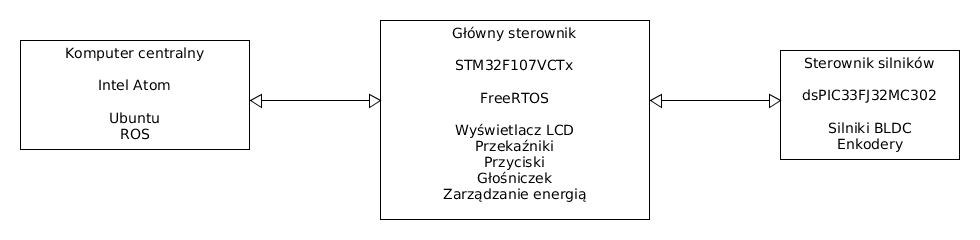
\includegraphics[width=0.95\textwidth]{budowa_ogolna}
	    \caption{Ogólna budowa modułów decyzyjnych robota, wraz z podłączonymi do nich czujnikami i efektorami}
	    \label{img:budowaOgolna}
	\end{figure}

	\section{Łączność pomiędzy komputerem centralnym a głównym sterownikiem}
	Po wstępnym poznaniu sprzętu zostały wyspecyfikowane dodatkowe założenia pracy. Transmisja danych odbywać się będzie między UART4 mikrokontrolera, a portem RS-232 komputera centralnego, przy pomocy konwertera napięć MAX3232. Prędkość transmisji to 115200bit/s. Jest wystarczająca, aby zmieścić się w narzuconym reżimie czasowym, a jednocześnie nie powoduje zbyt dużo błędów transmisji. Transmisja jest ośmiobitowa, bez bitów parzystości. Aby zapewnić poprawność danych wysyłane struktury opakowywane są w ramki, zgodnie ze standartem High-Level Data Link Control, zatwierdzonym w jednej z norm ISO. Komputer centralny wysyła do głównego sterownika strukturę TxFrame inicjując komunikację. W odpowiedzi wysłane zostają dane zgodne ze strukturą RxFrame. Struktury mają pola opisane poniżej.
	\begin{lstlisting}
typedef struct 
{
	uint32_t timestamp;
	int16_t left_speed;
	int16_t right_speed;
	uint8_t relays;
	uint8_t sound;
	uint8_t shutdown;
}TxFrame;

typedef struct
{
	uint32_t timestamp;
	uint8_t buttons;
	int32_t left_position;
	int32_t right_position;
	uint16_t battery;
	uint8_t error;
}RxFrame;
	\end{lstlisting}
	Dzięki dodaniu pola timestamp istnieje możliwość łatwego pomiaru czasu całej transmisji, wraz z przetwarzaniem danych przez mikrokontroler.\par Po przesłaniu sterowania do głównego sterowania, najpierw następuje dalsze przesłanie danych sterujących do silników. W trakcie oczekiwania na odpowiedź, mikrokontroler głównego sterowania obsługuje inne urządzenia. Dopiero w chwili, gdy odebrane zostaną dane z enkoderów, oraz obsłużone zostaną inne urządzenia, do komputera centralnego odsyłany jest pakiet zawierający najświeższe dane. Cały proces obrazuje rysunek \ref{img:komunikacjaCzasowa}. Schemat tej architektury modeluje rysunek \ref{img:komunikacja}. 
	\begin{figure}[ht]
	    \centering
	    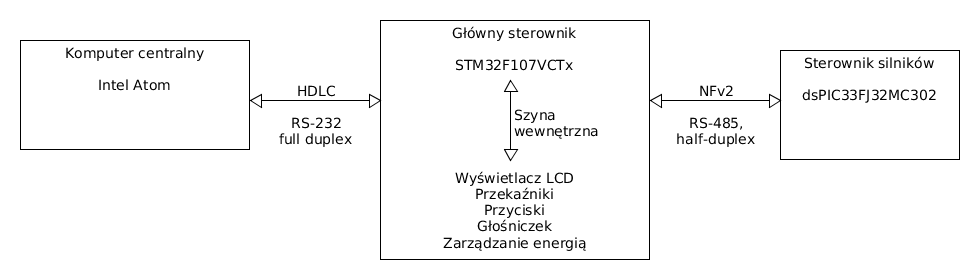
\includegraphics[width=0.95\textwidth]{schemat_komunikacji}
	    \caption{Schemat przedstawiający architekturę komunikacji pomiędzy urządzeniami robota}
	    \label{img:komunikacja}
	\end{figure}
	\begin{figure}[ht]
	    \centering
	    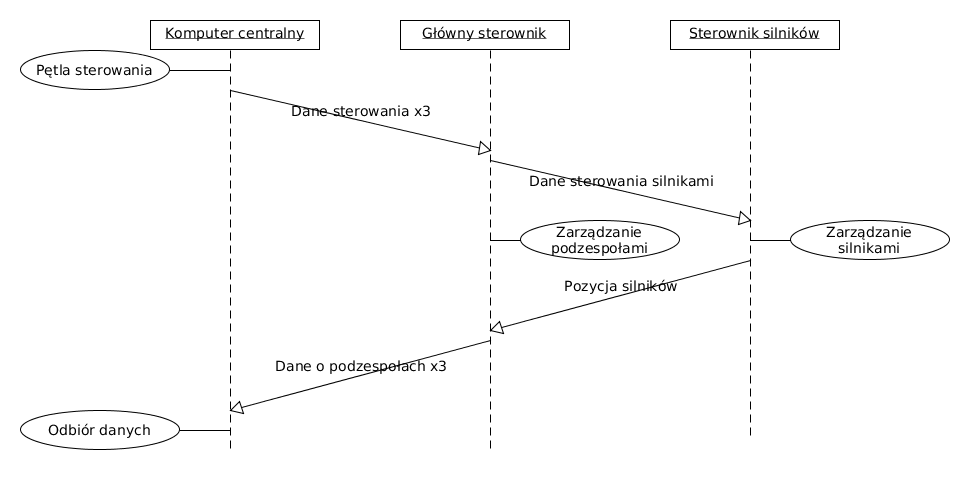
\includegraphics[width=0.95\textwidth]{schemat_komunikacji_czasowy.png}
	    \caption{Szczegółowy schemat komunikacji, z uwzględnieniem zależności czasowych}
	    \label{img:komunikacjaCzasowa}
	\end{figure}
	\section{Opis wykonanych czynności}
	\subsection{Uruchomienie mikrokontrolera STM32F107}
	Autor pracy nigdy wcześniej nie programował mikrokontrolerów tej firmy. Pewien czas został więc spożytkowany na wdrożenie się w dokumentację mikrokontrolera, oraz wybór środowiska programistycznego. W trakcie rozpozania został skonfigurowany debbuger wraz z programatorem ST-Linkv2. Skonfigurowano też system FreeRTOS w wersji ósmej. Na tym etapie dużym ułatwieniem było skorzystanie z oprogramowania ze strony producenta, czyli aplikacji CubeMX oraz SystemWorkbech. Uruchomiono podstawowe urządzenia peryferyjne mikrokontrolera z wykorzystaniem biblioteki HAL.
	\subsection{Uruchomienie wyświetlacza LCD}
	Wyświetlacz zamontowany w robocie Elektron ma sterownik KS0108. Ma rozdzielczość 128x64 pikseli i jest monochromatyczny.
	\subsection{Uruchomienie portu Ethernetu}
	Niestety ta czynność nie została zakończona sukcesem. Mimo usilnych starań, oraz zastosowania się do zaleceń producenta mikrokontroler stale zawieszał się na konfiguracji DMA Ethernetu. Pewną poszlaką w diagnozie zaistniałej sytuacji może być lektura erraty opisującej mikrokontroler, znajdująca się na stronie producenta. Wynika z niej, że mikrokontroler dokładnie w tej rewizji w której był używany, może faktycznie mieć błąd w konfiguracji DMA Ethernetu. Jednak według tej erraty mikrokontroler zachowywać się niepoprawnie, tylko jeśli wcześniej był usypiany, a fakt ten nie miał miejsca\cite{STMErrata}. Inne możliwe przyczyny niedziałania to błąd w projekcie sterownika, powodujący zakłócenia elektromagnetyczne, albo zwyczajna omyłka programisty. Wykluczone zostały jednak ewentualne uszkodzenia fizyczne, poprzez programowanie takiego samego sterownika w robocie Elektron 2. Autor pracy z ciekawości uruchomił port Ethernetu na płytce Nucleo z mikrokontrolerem STM32F207, z tym samym co w STM32F107 rdzeniem Cortex M3, bez większych problemów. Brak możliwości komunikacji w ten sposób spowodował zmianę założeń pracy.
	\subsection{Uruchomienie silników}
	Wykorzystując bibliotekę NFv2 dostarczoną do sterownika silników udało się zarówno zadawać prędkość jak i uzyskać odczyt danych z enkoderów. Połączenie ze sterownikiem silników odbywa się poprzez USART2 mikrokontrolera STM32F107, z prędkością 5600bit/s. Wykorzystywany jest do tego standard RS485 w trybie half-duplex. Dokonano też niewielkich modyfikacji w kodzie sterownika silników, co w przyszłości może owocować stabilniejszą pracą sterownika.
	\subsection{Przyciski i przekaźniki}
	Przekaźniki są sterowane, przez porty GPIO mikrokontrolera, za pomocą tranzystorów. Także przyciski są obsługiwane w ten sposób. Do odczytu stanu przycisków zastosowano algorytm cyfrowej eleminacji drgań.
	\subsection{Pomiar napięcia baterii}
	Realizowany jest poprzez przetwornik ADC mikrokontrolera.
	\subsection{Prace serwisowe}
	W trakcie użytkowania wykonano przegląd okablowania, wymieniono na nowy dysk twardy, oraz niedziałający układ MAX3485, umieszczony w sterowniku silników.
	\subsection{Implementacja łączności}
	Została wykonana, poprzez napisane biblioteki dla systemu Linux, udostępniającej API zgodne z wcześniejszymi założeniami. Drugą czynnością wykonaną w ramach zadania było napisanie odpowiedniego programu dla głównego sterownika, współpracującego z tą biblioteką. W ramach tego zadania uruchomiono port RS-232 na obu urządzeniach.
	
	\section{Program głównego sterownika}
	Program pisany był, przy wykorzystaniu biblioteki HAL, oraz systemu czasu rzeczywistego FreeRTOS. Składa się on z kilku zadań, z których najważniejsze odpowiadają za komunikację ze sterownikiem silników i komputerem centralnym. Implikacją tego faktu jest zastosowanie różnych priorytetów dla poszczególnych z zadań.

	\section{Opis planowanych działań}
	Autor pracy uważa, że ogólny stan prac jest dobry. Została wykonana najważniejsza część pracy, czyli funkcjonująca biblioteka dla systemu Ubuntu, wraz z odpowiednim programem dla głównego sterownika robota. Pozostało jednak jeszcze kilka zadań.
	\begin{enumerate}
		\item Integracja biblioteki z ROSem.
		\item Implementacja prostej aplikacji demonstrującej działanie łączności.
		\item Testy przedstawionego rozwiązania. 
		\item Zainstalowanie nowego oprogramowania i ewentualna adaptacja sprzętu w robotach Elektron 1 i Elektron 2. \
	\end{enumerate}
	\bibliography{thebibliography} 
	\bibliographystyle{ieeetr}
\end{document}
